\documentclass{beamer}

\usepackage[british]{babel}
\usepackage{graphicx,hyperref,ru,url}

\title[AI@Webscale Presentation]{
  AI at the Webscale Project Results}

\author[Bas Bootsma, Fenno Vermeij]{Bas Bootsma \& Fenno Vermeij}

\institute[Radboud University Nijmegen]{Radboud University Nijmegen}

\date{\today}

\begin{document}

\begin{frame}
  \titlepage
\end{frame}

\begin{frame}
	\frametitle{Approach}	
	\begin{itemize}
		\item Epsilon-greedy
		\item Gibbs-sampling
		\item Thompson-sampling
	\end{itemize}
\end{frame}

\begin{frame}
	\frametitle{Model}
	\begin{itemize}
		\item $r = \beta_0 + \beta_1 c_1 + \ldots + \beta_k c_k + \beta_{k+1} a_1 + \ldots + \beta {k+l} a_l + \beta_{x_1} c_1a_1 + \ldots + \beta_{x_m} c_ka_l$
		\item For reward: use price $\times$ effect instead of effect
	\end{itemize}
\end{frame}

\begin{frame}
	\frametitle{Visualization}
	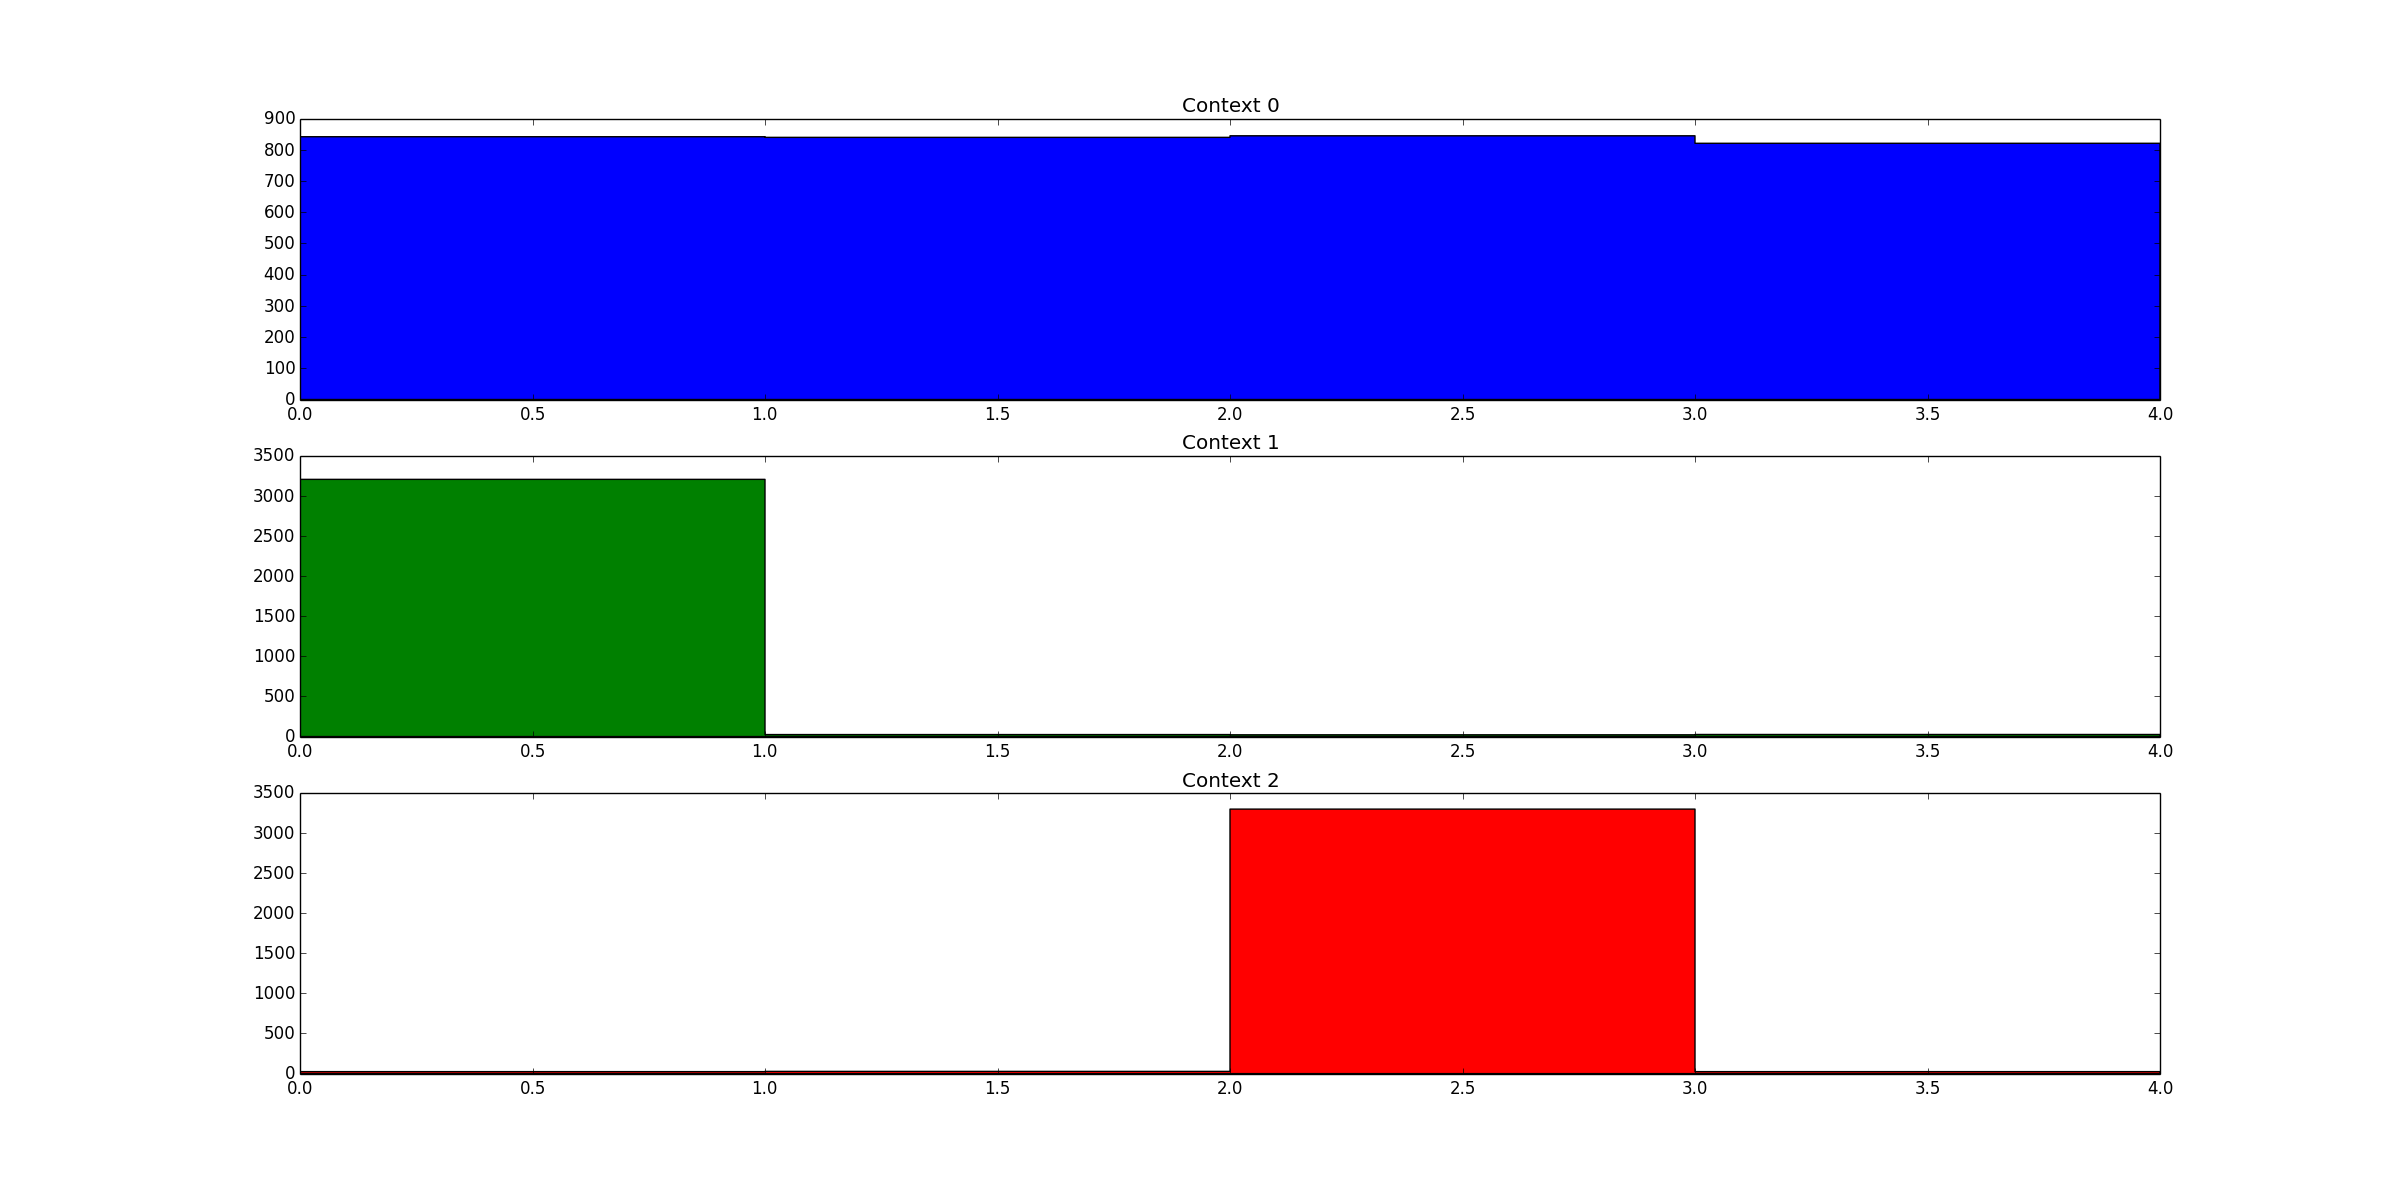
\includegraphics[width=\textwidth]{test.png}
\end{frame}

\begin{frame}
	\frametitle{Visualization}
	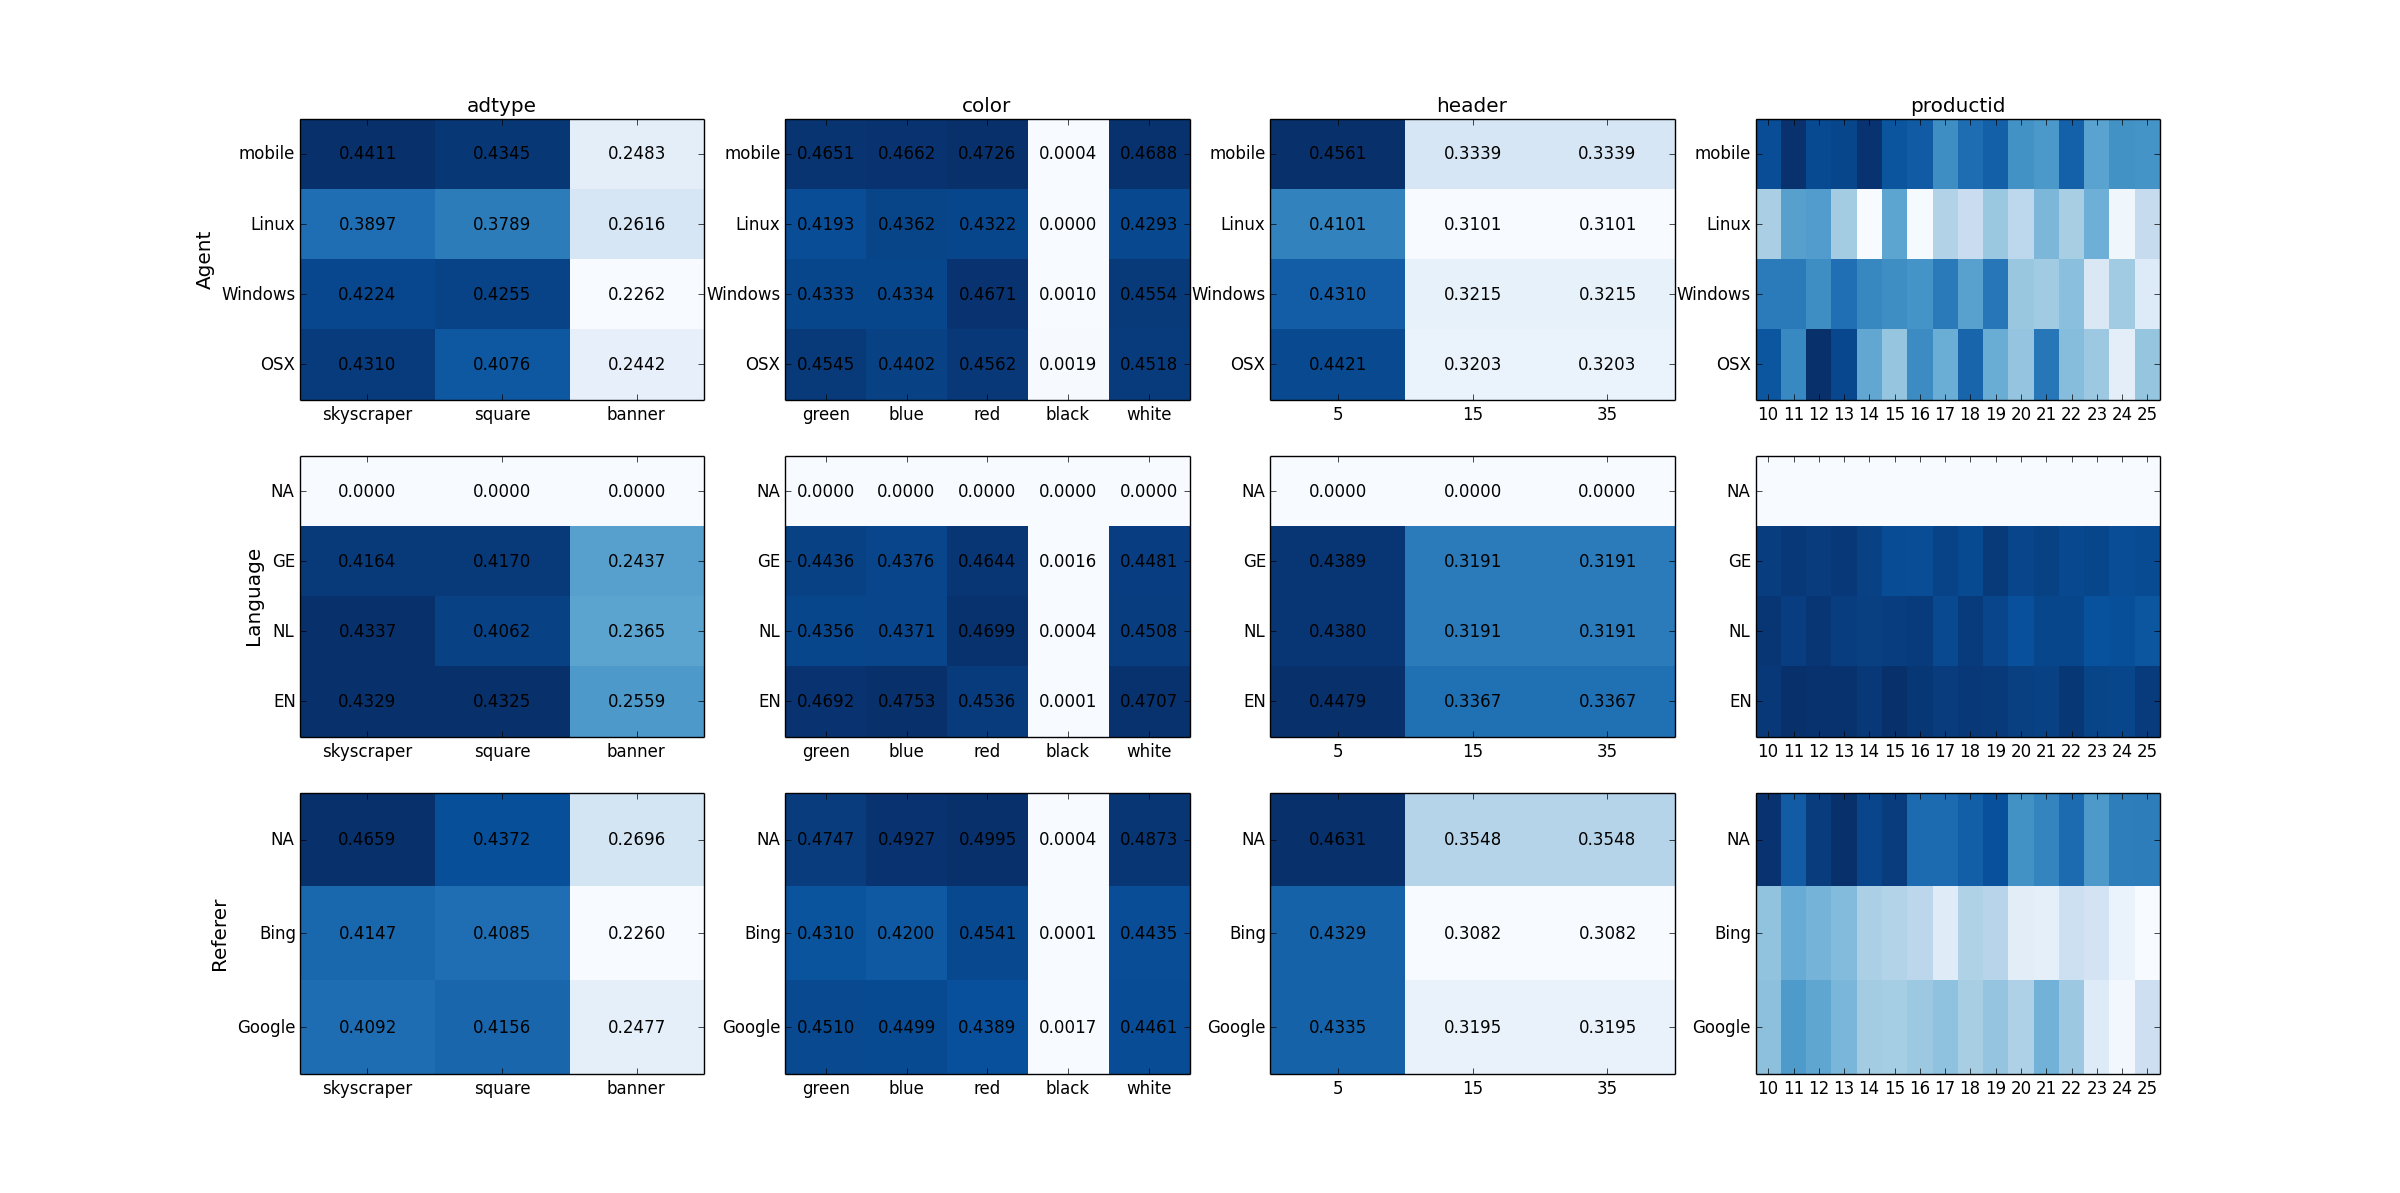
\includegraphics[width=\textwidth]{viewer.png}
\end{frame}


\begin{frame}
	\frametitle{Misc. Improvements}
	\begin{itemize}
		\item Price: in buckets: [1, 5, 10, 15, 20, 25, 30, 35, 40, 45, 50]
		\item Multivariate Gaussian speedup: use Cholesky transformation
		\item Userid: add extra features: average price user paid previously, if user has bought anything previously
	\end{itemize}
\end{frame}


\begin{frame}
  \frametitle{Results}

  \begin{itemize}
    \item Average reward: 
    \item Standard deviation: 
    \item Any questions?
  \end{itemize}
\end{frame}

\end{document}
